\section{Windfall of malice}

In the previous section we experienced the havoc a malicious player is capable of causing in a congestion game.
But is the opposite possible -- that there is an improvement by the malicious player?
After all, there are many paradoxes of this kind in game theory.
In this section we will see that there is indeed a \emph{Windfall of Malice}, but first we will take a look at \emph{Breass' paradox} to construct, and understand the nature of, that paradox.

\subsection{Braess' paradox}

Braess' paradox was discovered by Dietrich Braess in 1968 and demonstrates how an additional strategic option is able to cause a worse stable solution in a congestion game than before.
In Figure \ref{braess-base} we see a congestion game.
Because of its symmetry, the Nashflow is divided in two equal parts -- on the upper path flows 1/2 and on the lower one, too.
The resulting Nashdelay is thus 1.25.
In the real world, we could interpret this game as a street network where daily people commute from $s$ to $t$ and the nashdelay is the length of a traffic jam.

If the city council however decides to add an additional road between $p$ and $q$ (see \ref{braess-complete}) to decrease the congestion, they achieve the opposite -- the nashdelay increases because nash flow only uses the path $s-p-q-t$.
But why?
Because the delay of the upper and of the lower path are always bigger than the delay of the central path:
Let $P$ be the upper path $s-p-t$ and $P^*$ the central path $s-p-q-t$.
Because the flow value is $v=1$ the load of an edge cannot exceed 1.
\begin{align*}
	L(P) = f(e_1)/2 + 1 \geq f(e_1)/2 + f(e_2)/2 + f(e_3)/2 = L(P^*) 
\end{align*}
By symmetry this also holds for the lower path.
And because the old nash flow is not stable anymore, the only nash flow is that one which concentrates all on $P^*$.
But the nash delay is here $L(P^*) = 1.5$.

\begin{figure}
	\subfloat[Congestion game with flow value $v=1$\label{braess-base}]{
		\begin{tikzpicture}[scale=0.7]
			\SetGraphUnit{2}
			\GraphInit[vstyle=Classic]
			\SetUpEdge[style={->, thick}, color=gray]
			\tikzset{LabelStyle/.style = {fill=none, sloped, above}}
			
			% Knoten
			\Vertices[unit=3]{circle}{t,p,s,q}
			
			% Kanten
			\Edge[label=$x/2$](s)(p)
			\Edge[label=$x/2$](q)(t)
			\Edge[label=$1$](s)(q)
			\Edge[label=$1$](p)(t)
		\end{tikzpicture} 
	}
	\subfloat[adding the shortcut\label{braess-complete}]{
		\begin{tikzpicture}[scale=0.7]
			\SetGraphUnit{2}
			\GraphInit[vstyle=Classic]
			\SetUpEdge[style={->, thick}, color=gray]
			\tikzset{LabelStyle/.style = {fill=none, sloped, above}}
			
			% Knoten
			\Vertices[unit=3]{circle}{t,p,s,q}
			
			% Kanten
			\Edge[label=$x/2$](s)(p)
			\Edge[label=$x/2$](q)(t)
			\Edge[label=$1$](s)(q)
			\Edge[label=$1$](p)(t)
			% Abkürzung
			\Edge[label=$x/2$](p)(q)
		\end{tikzpicture}
	}
	\caption{Example network for Braess' paradox, first without, then with the shortcut. The Nashdelay increases form 1.25 to 1.5.}
\end{figure}

But before we are able to proceed to the windfall of malice we have to make a small adjustment of the congestion game above.
We replace the edge $p-q$ with a slightly more complex subgraph (see \ref{braess-modified}). 
But this subgraph behaves exactly like the edge:
Let there be a nash flow with flow value $u$ between $p$ and $q$.
Then it is divided equally between the path $p-m-q$ and $p-n-q$ and thus has a nash delay of $u/2$ -- exactly like a nash flow between $p$ and $q$ in the old network.
\begin{marginfigure}
	\begin{tikzpicture}[scale=0.7]
	\SetGraphUnit{2}
		\GraphInit[vstyle=Classic]
		\SetUpEdge[style={->, thick}, color=gray]
		\tikzset{LabelStyle/.style = {fill=none, sloped, above}}
		
		% Knoten
		\Vertices[unit=3]{circle}{t,p,s,q}
		
		% Kanten
		\Edge[label=$x/2$](s)(p)
		\Edge[label=$x/2$](q)(t)
		\Edge[label=$1$](s)(q)
		\Edge[label=$1$](p)(t)
		
		%innen
		\EA[Lpos=180](s){m}
		\EA[unit=2](m){n}
		\Edge[label=$0$](p)(n)
		\Edge[label=$0$](m)(n)
		\Edge[label=$0$](m)(q)
		\Edge[label=$x$](p)(m)
		\Edge[label=$x$](n)(q)
	\end{tikzpicture}
	\caption{Modified network which has also a nash delay of 1.5}
	\label{braess-modified}
\end{marginfigure}


\subsection{Reverting Braess' paradox with the malicious player}

After discussing Braess' paradox we address the windfall of malice.
What happens if we add a malicious player to the game above?
We see a \emph{decrease} of the nash delay!
In some manner, the windfall of malice counteracts Braess' paradox.

To analysis this behaviour, we first determine the malicious best response.
The \textsc{Mbr} is always the path $s,p,m,n,q,t$ because this covers all edges with non-constant latency functions (similar like in the section before).
\begin{figure}
	\begin{tikzpicture}[scale=0.7]
	\SetGraphUnit{2}
	\GraphInit[vstyle=Classic]
	\SetUpEdge[style={->, thick}, color=gray]
	\tikzset{LabelStyle/.style = {fill=none, sloped, above}}
	
	% Knoten
	\Vertices[unit=3]{circle}{t,p,s,q}
	\EA[Lpos=180](s){m}
	\EA[unit=2](m){n}
	
	% Kanten
	\Edge[label=$1$](p)(t)
	\Edge[label=$0$](p)(n)
	\SetUpEdge[style={->, thick}, color=myRed]
	\tikzset{LabelStyle/.style = {fill=none, sloped, above}}
	\Edge[label=$x/2$](s)(p)
	\Edge[label=$x$](p)(m)
	\Edge[label=$0$](m)(n)
	
	\SetUpEdge[style={->, thick}, color=gray]
	\tikzset{LabelStyle/.style = {fill=none, sloped, below}}
	\Edge[label=$1$](s)(q)
	\Edge[label=$0$](m)(q)
	\SetUpEdge[style={->, thick}, color=myRed]
	\tikzset{LabelStyle/.style = {fill=none, sloped, below}}
	\Edge[label=$x$](n)(q)
	\Edge[label=$x/2$](q)(t)
	
	
	\end{tikzpicture}
	\caption{Game with a malicious player's \textsc{Mbr} drawn in with red colour.}
	\label{wof-mbr}
\end{figure} 
